Data analysis in the context of this project is completed as a series of stages, each of which consists of a sequential process of ETL, followed by querying and analysis. Figure \ref{analysis-workflow} shows the sequential steps involved in a single stage of analysis; nETL is executed with a configuration file specifying CSV extraction, transformations, and the destination database as a parameter, CouchDB builds a view-index according to the MapReduce view as specified via a design document, data is retrieved via a List function also specified on the design document, and subsequent analyses (stages) are performed in context of the proceeding stages results. For each stage in the analysis, the configuration of nETL is discussed in terms of logical operations, and the configuration files themselves are included in the appendix (see \ref{netl-configuration}).

With the eventual aim of assessing the relationships between LMS usage and course grades, the following series of analyses is conducted in terms of the CSC1015F course.

\begin{enumerate}
    \item \textit{Stage 1}: Assessing effectiveness of different benchmarking formulas using the Benchmarks data
    \item \textit{Stage 2}: Assessing the correlation between Events and Grades data
    \item \textit{Stage 3}: As a means of control, assessing the correlation between Events and Benchmarks
    \item \textit{Stage 4}: Assessing the relationship of student performance relative to their peers as benchmarked compared to course performance, in terms of LMS usage
\end{enumerate}
\begin{figure}[]
    \centering
    \begin{mdframed}
        \centering
        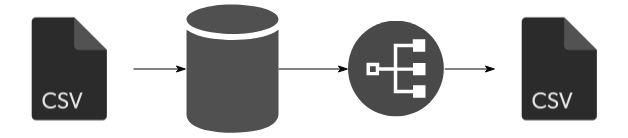
\includegraphics[scale=0.35]{./resources/figures/analysis.png}
    \end{mdframed}
    \caption[Analysis Workflow]{\textbf{Figure \ref{analysis}: Workflow to perform an analysis.} The analysis process represented as a simple pipeline. First nETL extracts data from CSV files and loads that into a CouchDB database via the CouchDB server API. This file consists of a B+tree organized by the \_id field of each document created as a UUID on document write by CouchDB to guarantee uniqueness of every document. From the database file an index is created, also structured as a B+tree but organized by a key as a specified in the Map Function. This allows for sorted output according to a users requirements. A List function is used to retrieve the contents of the view, transform those contents into tabular (CSV) form. The result of calling the List function is a downloaded CSV file. The List function address (API) is of the form \texttt{http(s)://<host>:<port>/<db>/\_design/<doc>/\_list/<fn>/<view>?<params>}}
    \label{analysis}
\end{figure}

In addition to outlining a structured approach by which the results are obtained for CSC1015F, further discussion is provided on how multiple courses may be analyzed simultaneously via more advanced usage of CouchDB's MapReduce implementation. During analysis, runtime results of the different components of the system are recorded and are shown in Table \ref{performance-analysis}. The metrics include running time of nETL tasks, a summary of the data processed by nETL, CouchDB indexing times, and database/index storage footprints.

In terms of defining MapReduce tasks, the map function is always user-defined, whereas a built-in reduce function (\_stats) is always used. The built-in reduce function are implemented within the main Erlang process, which according to the documentation offers a performance boost since the IO transfer cost between the Erlang process and the view engine (couchjs.exe by default) is negated. Working on a Windows machine the IO cost is apparently exaggerated (see the slack correspondence with Jan Lehnardt in appendix \ref{slack-1-nov}) due to the difference between Unix-based and Windows kernel implementations.

\begin{table}[H]
    \begin{threeparttable}
        \textbf{Table \ref{tbl-grades-normalize}}\par\medskip\par\medskip
        \caption{Grade results need to be treated as numbers for the purpose of this analysis, this table shows all different value types and the appropriate treatment for each. Because of the volume of data, it was not checked how many of these symbols apply to undergraduate students specifically, so these cases were handled generically}
        \label{tbl-grades-normalize}
        \begin{tabularx}{\textwidth}{>{\hsize=0.6\hsize}X>{\hsize=1.3\hsize}X>{\hsize=1.1\hsize}X}
            \toprule
            \mC{c}{Symbol} & \mC{c}{Meaning}          & \mC{c}{Handling Logic}                     \\
            \midrule
            49A            & Absent for supplementary & Grade used                                 \\
            49S            & Supplementary pending    & Grade used                                 \\
            50C            & ?                        & Grade used                                 \\
            78             & Grade                    & Grade used                                 \\
            AB             & Absent (fail)            & N/A                                        \\
            ATT            & ?                        & N/A                                        \\
            DE             & Deferred                 & N/A                                        \\
            DPR            & Duly performed refused   & 30\% Grade used\tnote{\textsuperscript{1}} \\
            F              & Fail                     & 40\% Grade used\tnote{\textsuperscript{2}} \\
            GIP            & Thesis only              & N/A                                        \\
            INC            & Incomplete (fail)        & 30\% Grade used\tnote{\textsuperscript{1}} \\
            LOA            & Leave of absence         & N/A                                        \\
            OS             & Outstanding              & N/A                                        \\
            OSS            & Outstanding              & N/A                                        \\
            PA             & Pass (thesis)            & N/A                                        \\
            SAT            & Thesis only              & N/A                                        \\
            UF             & Unclassified Fail        & 49\% Grade used\tnote{\textsuperscript{3}} \\
            UNS            & Thesis only              & N/A                                        \\
            UP             & Unclassified pass        & 45\% Grade used\tnote{\textsuperscript{4}} \\
            \bottomrule
        \end{tabularx}
        \scriptsize
        \begin{tablenotes}
            \item[\textsuperscript{1}]30\% was applied on the estimate that these students wouldn't necessarily have completed the coursework, and that as such this is a `bad' fail
            \item[\textsuperscript{2}]40\% was applied on the estimate that this symbol would apply to students who participated in the course but still failed
            \item[\textsuperscript{3}]49\% was applied on the estimate that this is a `good' fail, in that the UF classification applies to borderline fails
            \item[\textsuperscript{4}]45\% was applied on the estimate that UP is the 'worst' pass, in that from a strictly grade perspective, these students technically failed
        \end{tablenotes}
    \end{threeparttable}
\end{table}
\begin{table}[H]
    \begin{threeparttable}
        \textbf{Table \ref{performance-analysis}}\par\medskip\par\medskip
        \caption[Software performance analysis]{Running time analysis of \textit{nETL} tasks and CouchDB MapReduce indexing}
        \label{performance-analysis}
        \begin{tabularx}{\textwidth}{>{\hsize=1.8\hsize}X>{\hsize=0.8\hsize}Y>{\hsize=0.8\hsize}Y>{\hsize=0.8\hsize}Y>{\hsize=0.8\hsize}Y}
            \toprule
            \mC{c}{}                                               & \mC{c}{2-Way Join} & \mC{c}{3-Way-join}             & \mC{c}{Variance} & \mC{c}{Tests} \\
            \midrule
            Demographic lines extracted                            & -                  & -                              & -                &               \\
            Demographic lines loaded                               & -                  & -                              & -                &               \\
            Demographic task time (sec)\tnote{\textsuperscript{1}} & -                  & -                              & -                &               \\
            \midrule
            Grade lines extracted                                  & -                  & -                              & -                &               \\
            Grade lines loaded                                     & -                  & -                              & -                &               \\
            Grade task time (sec)\tnote{\textsuperscript{1}}       & -                  & -                              & -                &               \\
            \midrule
            Events lines extracted                                 & -                  & 44 420 508                     &                  &               \\
            Events lines loaded                                    & -                  & -                              & -                &               \\
            Events task time (sec)\tnote{\textsuperscript{1}}      & -                  & -                              & -                &               \\
            \midrule
            CouchDB footprint (MB)\tnote{\textsuperscript{2}}      & -                  & -                              & -                &               \\
            View calculation time (sec)\tnote{\textsuperscript{3}} & -                  & -                              & -                &               \\
            View size (MB)                                         & -                  & -                              & -                &               \\
            \midrule
            List function output                                   & -                  & 586\tnote{\textsuperscript{4}} & -                & -             \\
            \bottomrule
        \end{tabularx}
        \scriptsize
        \begin{tablenotes}
            \item[\textsuperscript{1}]Tasks are run asynchronously, so time taken includes processing of other tasks in this run. Task run times are printed out to the log
            \item[\textsuperscript{2}]This is representative of the amount of data processed by \textit{nETL}
            \item[\textsuperscript{3}]CouchDB views are calculated per shard. By default a database contains 8 shards (even in single node mode). The log file shows start and end times of view calculations for each shard, the time is taken as time the first shard starts indexing, to the time the last shard stops indexing
            \item[\textsuperscript{4}]This file comprises a unique list of students, each student associated with the joined output.
        \end{tablenotes}
    \end{threeparttable}
\end{table}

\section{MapReduce Considerations}
Initial attempts at joining the three entities - Grades with Benchmarks, and then Grades with Benchmarks with Events were attempted directly via MapReduce (the custom Map and \_stats reduce function). This approach involved specifying the map function to always output a value of the same format for all three entities. This format is a tuple of [0, 0, 0, 0, 0, 0, 0, 0, 0, 0, 0]; each of the 11 indexes correlate to a specific output attribute. In other words, i = 0 (indexes in JavaScript start at 0) correlates to Grade \%, i = 1,2,3,4,etc. correlated to the percents for Benchmark data, and the last 2 indexes (i = 9, i = 10) indicate an event occurrence (from the Event data) in either the first semester (i[9] = 1, i[10] = 0) or the second semester (i[9] = 0, i[10] = 1).

During index calculation, CouchDB then iterates through every database document, passing each document to the Map function. This Map function instantiates the output tuple ([0, 0, 0, 0, 0, 0, 0, 0, 0, 0, 0]) on every execution, and then depending on the value of the `type\_' attribute of the document it's processing (this attribute is added to every document prior to insertion to CouchDB), the map function alters the tuple at certain indexes before returning and adding the key:value set to the view index currently being built.

To further explain, if the document being processed by the map function is a ‘grade’ document, then the map function adjusts the value tuple to emit the grade percent – i.e. [percent, 0, 0, 0, 0, 0, 0, 0, 0, 0, 0]. Or if the document is of type ‘demographic’, the map function changes the values at indexes 2 through 9 and emits the value: [0, x, x, x, x, x, x, x, x, 0, 0]. If the document is of type ‘event’, then the map function alters the value at indexes 9 and 10. i.e. [0, 0, 0, 0, 0, 0, 0, 0, s1Event, s2Event] (s1Event is 1 for first semester event, or 0 for second semester, etc.).

The reduce function (whether that is the \_stats function a used in this study or any other function) then receives a tuple of tuples (a list of the tuples output by the map function executions), as the output per key, and can perform calculations across corresponding indexes; i.e. a single key references a list of 6 tuples: 1 Grade document output, 1 Benchmark document output, and 4 Event document outputs. By performing an aggregation across these 6 tuples at corresponding indexes, the Grades percentage (i=1) is an aggregation of the grade as output from the Grade entity along with five 0s, the Benchmark percentages are each aggregations of the Benchmark percent each along with five 0s, and the Events data is an aggregation of four event counts and two 0s. As such, aggregation across the output tuple effectively only takes into account relevant values (since all other values are 0) and a join is achieved.

However, for this approach to work, the reduce function needs to be able to group by common keys. To perform a grouping on the compound key [Student ID, Course, Course Year], all the entities need to output data in this format; but the Events data doesn't include Course, and the the Benchmarks data doesn't include Course or Course Year. As such, to allow for Grade data to be joined to Benchmark data on Course and Course Year in addition to Student ID, each Benchmark document needs to be output for every possible combination of Course and Course Year per student. That is the same with the Events documents - each Event needs to be output for every possible course that a student took in a given year.

In terms of performance this approach is disastrous. To analyze 40 courses taken over 3 years, each Benchmark document needs to be emitted for a student $40 x 3 = 120$ times so that the key of the Grade document [Student ID, Course, Year] can always be joined to Benchmark document. Likewise, Each Event data (which has year but not course information) needs to be emitted 40 times - once for each course a join could potentially be performed on. Considering that there are several million event documents this is impracticable.

Instead, CouchDB's usage of B+trees as a means of sorting view indexes by keys is utilized to allow for joining the 3 documents in the final dataset. Figure \ref{mapreduce-key-output} shows the key format for each type of document the Map function processes (Grade, Event, Benchmark). Keys are defined so that the index produced by the Map function is always ordered per particular student: i.e. for a particular Student ID, and scanning the B+tree, the first document found will be the Benchmark document, followed by Event document, and followed by Grade documents. The reduce function is then used to create an aggregation of all the event documents so that retrieval from the reduced view-index, for any student ID, iteratively produces first a Benchmark document, then a single (aggregated) Event document, then a single Grade document for each course that student enrolled in. This results in a much more efficient way of aggregating different types of documents for a given set of keys than was first attempted.

With ordered output, and Event data already aggregated via the reduce function, data retrieval involves iterating over view indexes, processing a single ID at a time. This is very efficient in terms of memory usage since only documents relating to a single ID need to be held in memory at a time.

\begin{figure}[H]
    \centering
    \begin{mdframed}
        \centering
        \begin{verbatim}
// Map output
[<ID>, ‘0’, 1]: [0, b1, b2, b3, b4, b5, b6, b7, b8, 0, 0]
[<ID>, ‘0’, <Year>]: [0, 0, 0, 0, 0, 0, 0, 0, 0, 1, 0]
[<ID>, ‘0’, <Year>]: [0, 0, 0, 0, 0, 0, 0, 0, 0, 1, 0]
[<ID>, ‘0’, <Year>]: [0, 0, 0, 0, 0, 0, 0, 0, 0, 0, 1]
[<ID>, ‘0’, <Year>]: [0, 0, 0, 0, 0, 0, 0, 0, 0, 0, 1]
[<ID>, ‘0’, <Year>]: [0, 0, 0, 0, 0, 0, 0, 0, 0, 0, 1]
[<ID>, ‘0’, <Year>]: [0, 0, 0, 0, 0, 0, 0, 0, 0, 1, 0]
[<ID>, ‘CSC1015F’, <Year>]: [98, 0, 0, 0, 0, 0, 0, 0, 0, 0, 0]
[<ID>, ‘MAM100F, <Year>]: [94, 0, 0, 0, 0, 0, 0, 0, 0, 0, 0]

// Resulting reduce output
[<ID>, ‘0’, 1]: [0, b1, b2, b3, b4, b5, b6, b7, b8, 0, 0]
[<ID>, ‘0’, <Year>]: [0, 0, 0, 0, 0, 0, 0, 0, 0, 3, 3]
[<ID>, ‘CSC1015F’, <Year>]: [98, 0, 0, 0, 0, 0, 0, 0, 0, 0, 0]
[<ID>, ‘MAM100F, <Year>]: [94, 0, 0, 0, 0, 0, 0, 0, 0, 0, 0]
        \end{verbatim}
    \end{mdframed}
    \caption[Aggregation By Sorted MapReduce output]{\textbf{Figure \ref{mapreduce-key-output}: Aggregating via a combination of MapReduce and relying on sorted B+tree keys.} The Map function should output keys in the form [ID, Course, Year] as shown above for all document processed. However this is not possible for document of type Benchmark (which don't include properties for Course or Year) or documents of type Events (which don't include the property Course). As such, a key of the required format is simply created so as to assure ordering of documents in the resultant B+tree index; in this case documents will all be ordered by Student ID, since all documents contain that property. For Benchmark data, the value `0' is emitted for Course since that value will result in the Benchmark data ordered before documents with a Course property. For the Year field, the value `1' is emitted for Benchmark data since that guarantees ordering of documents by year ahead of any real years. Likewise for documents of type Events, the value `0' is emitted for Course. The resultant B+tree index guarantees that for a particular ID, Benchmark output will occur before Event output which will occur before Grade output.}
    \label{mapreduce-key-output}
\end{figure}